\documentclass{article}
\setlength{\parindent}{0in}
\usepackage[
bottom = 2.50cm,
left   = 2.50cm,
right  = 2.50cm]{geometry}
\newcommand{\code}{\texttt}

\usepackage{graphicx}% Include fig. files
\usepackage{dcolumn}% Align table columns on decimal point
\usepackage{bm}% bold math
\usepackage{caption}
\usepackage[labelformat=simple]{subcaption}
\usepackage{float}
\usepackage{amsmath}
\usepackage{amssymb}
\usepackage[export]{adjustbox}
\usepackage[dvipsnames]{xcolor}
\usepackage{authblk}
\usepackage{url}
\usepackage{listings}
\usepackage{braket}

\begin{document}

\title{ESC407 Lab 2}

\author{Maggie Wang}

\date{October 16, 2023}
\maketitle

\begin{enumerate}
\item Central Differences for Numerical Differentiation
\begin{enumerate}
    \item The derivative of $f(x)=e^{2x}$ was calculated numerically at $x=0$, using central differences, as 
    \begin{align*}
        f'(x) &\approx \frac{f(x+h/2)-f(x-h/2)}{h}
    \end{align*}
    Table \ref{tab:1a} lists the numerically computed value of $f'(0)$ for different step sizes $h$ between $10^{-16}$ and $1$.
    
    % \begin{table}[h]
    %     \centering
    %     \begin{tabular}{c|c c c c c c}
    %         $h$ & $10^{-16}$ & $10^{-15}$ & $10^{-14}$ & $10^{-13}$ & 
    %         $10^{-12}$ \\ 
    %         $f'(0)$ & 1.11022302 & 2.10942375 & 1.99840144 & 1.99951167 &
    %         2.00006678 \\  [0.2 em] \hline  \\[-0.8em]
    %         $h$ & $10^{-11}$ & $10^{-10}$ & $10^{-9}$ & $10^{-8}$ & 
    %         $10^{-7}$ & $10^{-6}$ \\ 
    %         $f'(0)$ & 2.00000017 & 2.00000017 & 2.00000005 & 1.99999999 & 2. & 2. \\ [0.2 em] \hline  \\[-0.8em]
    %         $h$ & $10^{-5}$ & $10^{-4}$ & $10^{-3}$ & $10^{-2}$ & $10^{-1}$ & $10^{0}$\\
    %         $f'(0)$  & 2. & 2. & 2.00000033 & 2.00003333 & 2.003335 & 2.35040239
    %     \end{tabular}
    %     \caption{Derivative of $f(x)=e^{2x}$ at $x=0$ for different $h$ values}
    %     \label{tab:1a}
    % \end{table}

    \begin{table}[h]
        \centering
        \begin{tabular}{l l}
            $h$ & $f'(0)$\\ [0.2 em] \hline  \\[-0.8em]
            $10^{-16}$ & 1.1102230246251565 \\
            $10^{-15}$ & 2.1094237467877974 \\
            $10^{-14}$ & 1.9984014443252818 \\
            $10^{-13}$ & 1.9995116673499070 \\
            $10^{-12}$ & 2.0000667788622195 \\
            $10^{-11}$ & 2.0000001654807420 \\
            $10^{-10}$ & 2.0000001654807420 \\  
            $10^{-9}$ & 2.0000000544584395 \\
            $10^{-8}$ & 1.9999999878450580 \\
            $10^{-7}$ & 1.9999999989472883 \\
            $10^{-6}$ & 1.9999999999464890 \\
            $10^{-5}$ & 2.0000000000242046 \\
            $10^{-4}$ & 2.0000000033337795\\
            $10^{-3}$ & 2.0000003333333627\\
            $10^{-2}$ & 2.0000333334999842\\
            $10^{-1}$ & 2.0033350003968820\\
            $1$ & 2.3504023872876028\\
        \end{tabular}
        \caption{Derivative of $f(x)=e^{2x}$ at $x=0$ for different $h$ values}
        \label{tab:1a}
    \end{table}

    The raw output from the code is 
    \begin{verbatim}
1 a) errors
    h       f'(0)
    1e-16:	1.1102230246251565
    1e-15:	2.1094237467877974
    1e-14:	1.9984014443252818
    1e-13:	1.999511667349907
    1e-12:	2.0000667788622195
    1e-11:	2.000000165480742
    1e-10:	2.000000165480742
    1e-09:	2.0000000544584395
    1e-08:	1.999999987845058
    1e-07:	1.9999999989472883
    1e-06:	1.999999999946489
    1e-05:	2.0000000000242046
    0.0001:	2.0000000033337795
    0.001:	2.0000003333333627
    0.01:	2.0000333334999842
    0.1:	2.003335000396882
    1.0:	2.3504023872876028
    \end{verbatim}

    \item The expected optimal step size $h^*$ and corresponding error are calculated using equations (5.99) and (5.100) from the textbook, using $C=10^{-16}$. We find
    \begin{align*}
        h^* &= \bigg(24 C \bigg|\frac{f(x)}{f'''(x)}\bigg|\bigg)^{1/3}\\
            &= \bigg(\frac{24 C e^{2x}}{2^{3} e^{2x}}\bigg)^{1/3}\\
            &= \bigg(\frac{24 C}{2^3}\bigg)^{1/3}\\
            &\approx 6.7\times 10^{-6}
    \end{align*}
    and
    \begin{align*}
        \epsilon &= \frac{2C|f(x)|}{h^*} + \frac{1}{24}h^2|f'''(x)|\\
        &= 4.48\times10^{-11}
    \end{align*}
    
    The actual error is plotted against $h$ in fig \ref{fig:1b}. We see that the expected optimal step size and minimum in error are very close to their actual values.
    \begin{figure}[h]
        \centering 
        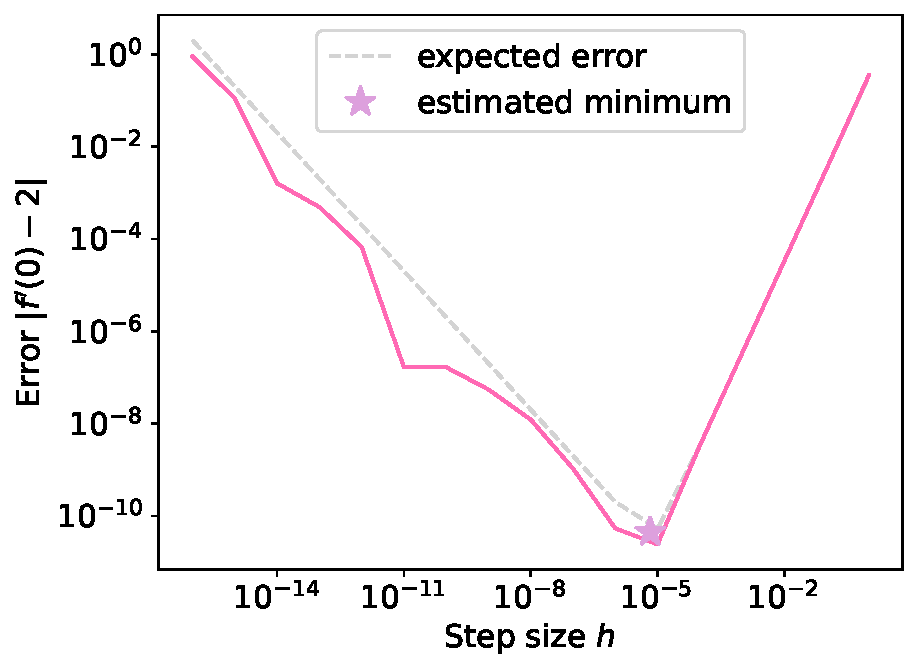
\includegraphics[width=0.5\textwidth]{Q1b.pdf}
        \caption{Calculated error of $f'(0)$ using central difference approximation vs step size $h$}
        \label{fig:1b}
      \end{figure}

    \item The first 10 derivatives of $f'(x)$ at $x=0$ were calculated using central differences, with higher derivatives implemented recursively. 
    Table \ref{tab:1c} lists the derivatives using the optimal step size from part b) (which is the same for all $m$), and with $h-0.05$.
    Using the optimal value of $h$, which is $\mathcal{O}(10^{-6})$, rounding error accumulate and calculated values of $f^m(0)$ diverges for $m>3$. 
    Using a larger $h$ reduces the roundoff error and leads to more accurate calculations the higher order derivatives.
    \begin{table}[H]
        \centering
        \begin{tabular}{l | c l l}
            $m$ & Analytical value & $h \approx 6.7\times10^{-6}$ & $h=0.05$\\ [0.2 em] \hline  \\[-0.8em] 
            1 & 2 & 2.0000000000234888 & 2.000833437506202\\
            2 & 4& 4.000001933007014 & 4.003334444642892\\
            3 & 8&7.77155789571232 & 8.010005418359611\\
            4 & 16&-221126.08039335813 & 16.02668667564089\\
            5 & 32&8258210993.557659 & 32.06673059601428\\
            6 & 64&2.2204420456714464e+16 & 64.16018684518576\\
            7 & 128&-3.68559504405105e+20 & 128.37384304020816\\
            8 & 256&-2.1195518363153336e+27 & 256.8546079828593\\
            9 & 514&2.05607099203305e+31 & 513.9293079992058\\
            10: & 1028&1.971716534777767e+38 & 1028.4099971613614\\
        \end{tabular}
        \caption{Approximate values for $f^m(0)$ computed using central differences, with step size $h=6.7\times10^{-6}$, and $h=0.05$.}
        \label{tab:1c}
    \end{table}
    % The optimal step size is the same for all $f^m(x)$:
    % \begin{align*}
    %     h^* &= \bigg(\frac{24 C f^m(x)}{f^{m+1}(x) }\bigg)^{1/3} \\ 
    %         &= \bigg(\frac{24 C \cdot 2^m e^{2x}}{2^{m+3} e^{2x}}\bigg)^{1/3}\\
    %         &= \bigg(\frac{24 C}{2^3}\bigg)^{1/3}\\
    %         &\approx 6.7\times 10^{-6}
    % \end{align*}
    The raw output from the code is:
\begin{verbatim}
1 c) derivatives using optimal h from part b: 
    m       optimal h                h=0.05
    1:      2.0000000000234888       2.000833437506202
    2:      4.000001933007014        4.003334444642892
    3:      7.77155789571232         8.010005418359611
    4:      -221126.08039335813      6.02668667564089
    5:      8258210993.557659        32.06673059601428
    6:      2.2204420456714464e+16   64.16018684518576
    7:      -3.68559504405105e+20    128.37384304020816
    8:      -2.1195518363153336e+27  256.8546079828593
    9:      2.05607099203305e+31     513.9293079992058
    10:     1.971716534777767e+38    1028.4099971613614
\end{verbatim}
\end{enumerate}

\item Integrating the Dawson Function Again
\begin{enumerate}
  \item Fig \ref{fig:2a} shows the Dawson function at $x=4$ evaluated using trapezoidal rule, Simpson's rule and Gaussian quadrature for varying integration slices $N$ between 8 and 2048 (where $N$ is always even for Simpson's rule). 
  The function calculated using Gaussian quadrature converges much more quickly than integration schemes using Newton-Cotes formulae.
  \begin{figure}[h]
    \centering 
    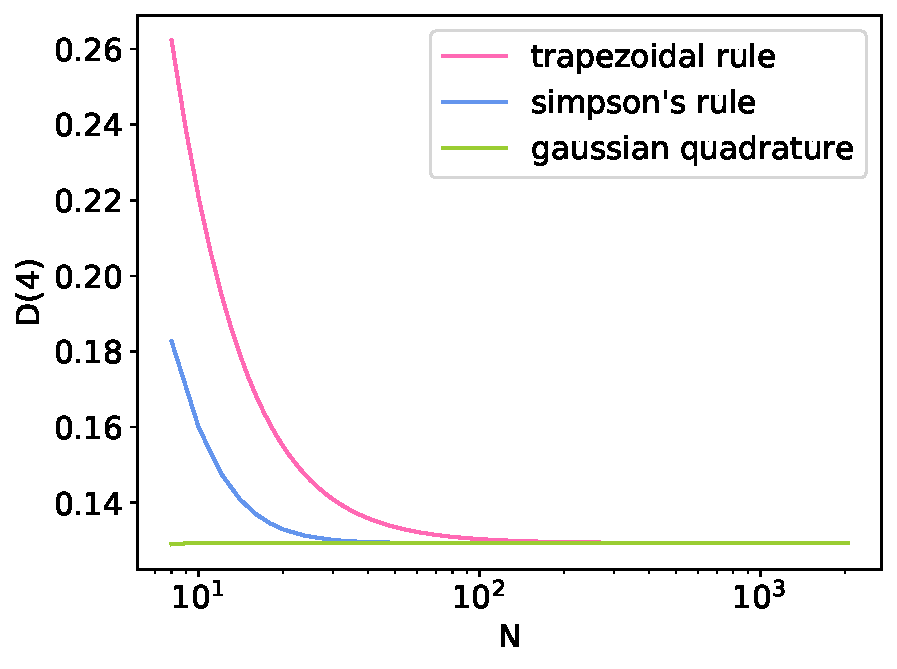
\includegraphics[width=0.4\textwidth]{Q2a.pdf}
    \caption{Dawson function $D(x)$ at $x=4$ calculated numerically vs number of integration slices $N$}
    \label{fig:2a}
  \end{figure}
  \item The error on $D(4)$ using Gaussian quadrature, $I_{2N} - I_N$ for the values of $N$ in 2a) are plotted in fig \ref{fig:2b}. The error decreases quickly from $N=8$ to around $N=20$, and then remains around the machine precision limit, 
  which suggests the accuracy is limited by roundoff error instead of estimations errors from using Gaussian guadrature.
  \begin{figure}[h]
    \centering 
    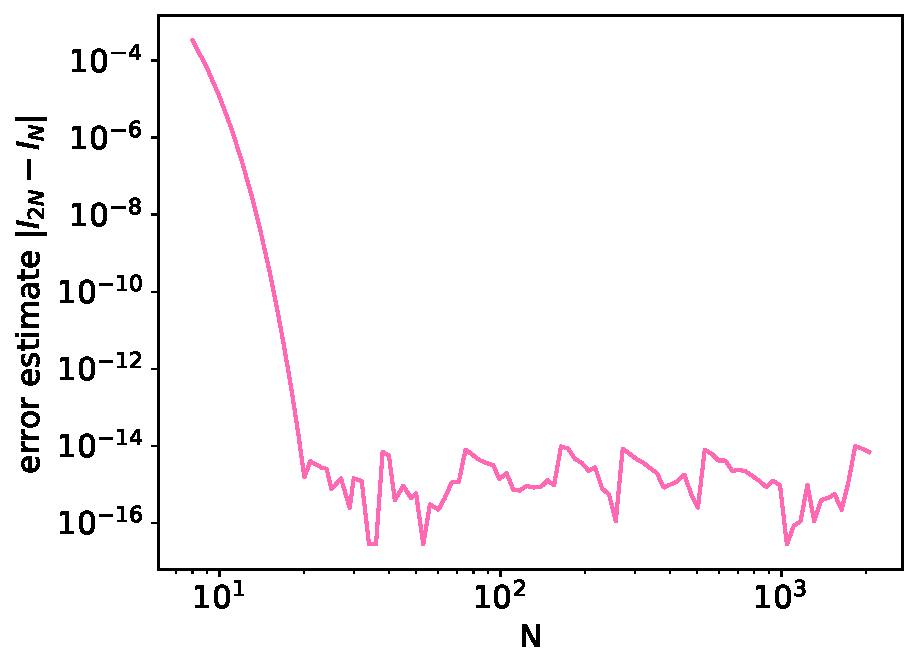
\includegraphics[width=0.42\textwidth]{Q2b.pdf}
    \caption{Error on $D(4)$ using Gaussian quadrature vs number of integration slices}
    \label{fig:2b}
  \end{figure}


  \item Fig \ref{fig:2c} shows the relative error on $D(4)$ calculated using Gaussian quadrature compared to the true value (from Scipy) as a function of the number of integration slices. 
  The behaviour of the relative error is the same as the estimated error from fig \ref{fig:2b}, while being around an order or magnitude larger than the estimated error.
  \begin{figure}[H]
    \centering 
    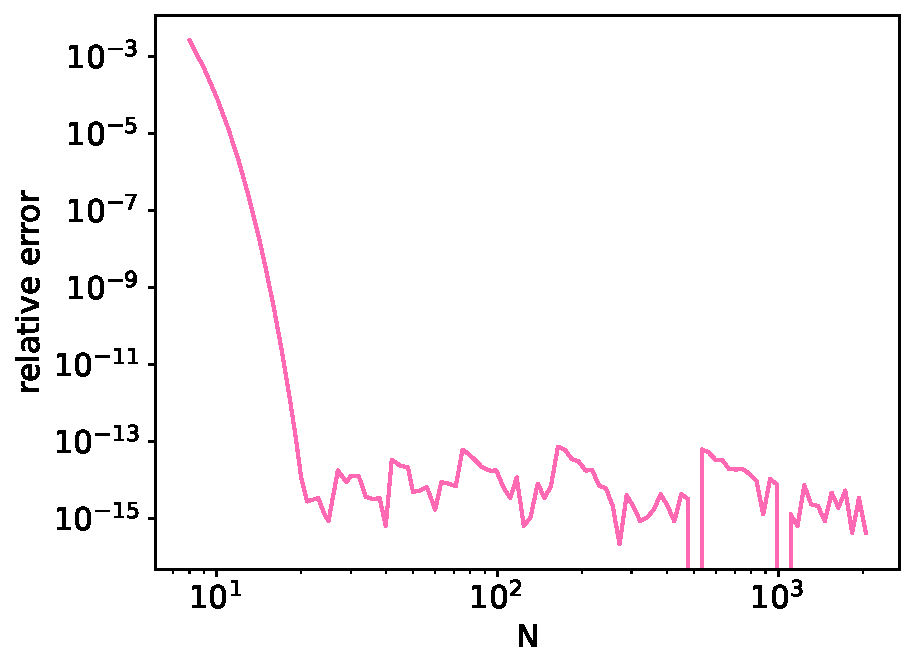
\includegraphics[width=0.42\textwidth]{Q2c.pdf}
    \caption{Relative error on $D(4)$ vs number of integration slices}
    \label{fig:2c}
  \end{figure}

\end{enumerate}

\item Calculating potential energy of QM harmonic oscillator 
\begin{enumerate}
    \item A function $H(n, x)$ was written to calculate the $n^{th}$ degree Hermite polynomial for a given x based on its recursion relation
    $H_{n+1}(x) = 2xH_n(x)-2nH_{n-1}(x)$.

    \item Fig \ref{fig:3b} shows the wave functions for the first 4 energy levels of a 1D quantum harmonic oscillator.
    \begin{figure}[H]
        \centering 
        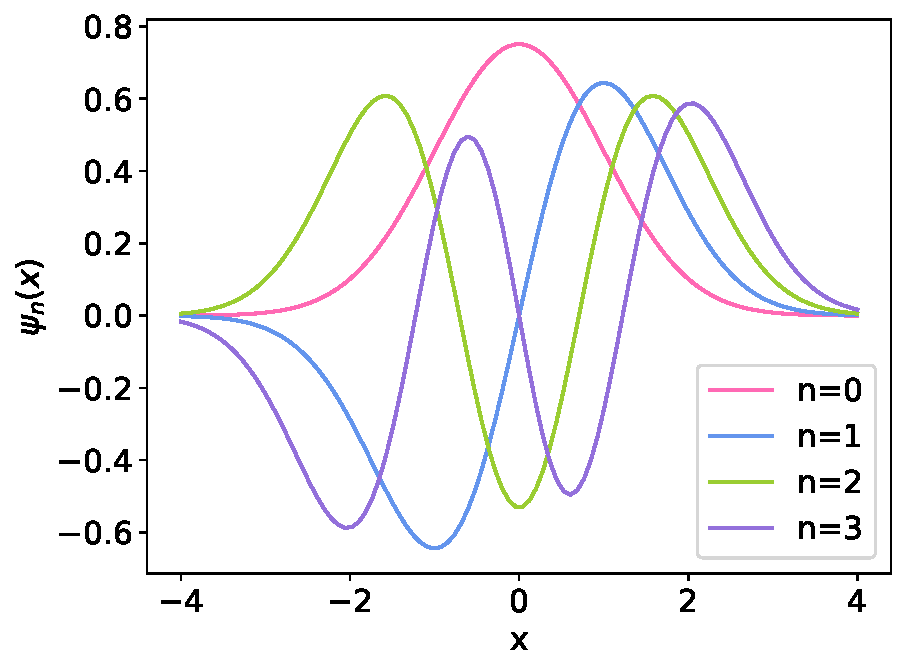
\includegraphics[width=0.42\textwidth]{Q3b.pdf}
        \caption{Harmonic oscillator wave functions}
        \label{fig:3b}
      \end{figure}

    \item The potential energy $U$ for $n$ from 0 to 10 computed using Gaussian quadrature using 100 points, from the formula 
    \begin{align*}
        U(n) &= \frac{\braket{x^2}}{2} = \int_{-\infty}^{\infty}x^2|\psi_n(x)|^2 dx
    \end{align*}

    The improper integral is treated by applying the following transformation
    \begin{align*}
        \int_{-\infty}^{\infty} f(x) dx &= \int_{-\pi/2}^{\pi/2} \frac{f(\text{tan }z)}{\text{cos}^2 z} dz
    \end{align*}
    Table \ref{tab:3c} lists the calculated potential energies of the particle for each $n$
    \begin{table}[h]
        \centering
        \begin{tabular}{c|c c c c c c c c c c c}
            $n$ & 0 & 1 & 2 & 3 & 4 & 5 & 6 & 7 & 8 & 9 & 10 \\
            $U(n)$ & 0.25 & 0.75 & 1.25 & 1.75 & 2.25 & 2.75 & 3.25 & 3.75 & 4.25 & 4.75 & 5.25
        \end{tabular}
        \caption{Potential energies of the quantum harmonic oscillator}
        \label{tab:3c}
    \end{table}

    The raw output from the code is 
\begin{verbatim}
0 0.24999999999999997
1 0.7500000000000119
2 1.2500000000003055
3 1.7499999999981126
4 2.249999999916142
5 2.7499999996902913
6 3.250000005587624
7 3.750000044358483
8 4.249999920351134
9 4.749998195042198
10 5.24999677662962
\end{verbatim}
\end{enumerate}

\end{enumerate}


\end{document}